\documentclass[border=12pt]{standalone}

\usepackage{amsmath,amssymb}
\usepackage{tikz}
\usetikzlibrary{arrows.meta,positioning,fit,backgrounds,calc}

\newcommand{\Set}{\mathbf{Set}}

% Palette (brand-neutral, readable in light & dark)
\definecolor{synth}{HTML}{2563EB}   % synthesis  (blue)
\definecolor{reason}{HTML}{059669}  % reasoning   (green)
\definecolor{classc}{HTML}{7C3AED}  % classify    (violet)
\definecolor{leak}{HTML}{DC2626}    % leak / bad  (red)
\definecolor{ink}{HTML}{111827}
\definecolor{mute}{HTML}{6B7280}
\definecolor{synthbg}{HTML}{EFF4FF}
\definecolor{reasonbg}{HTML}{ECFDF5}
\definecolor{classbg}{HTML}{F5F0FF}

\begin{document}
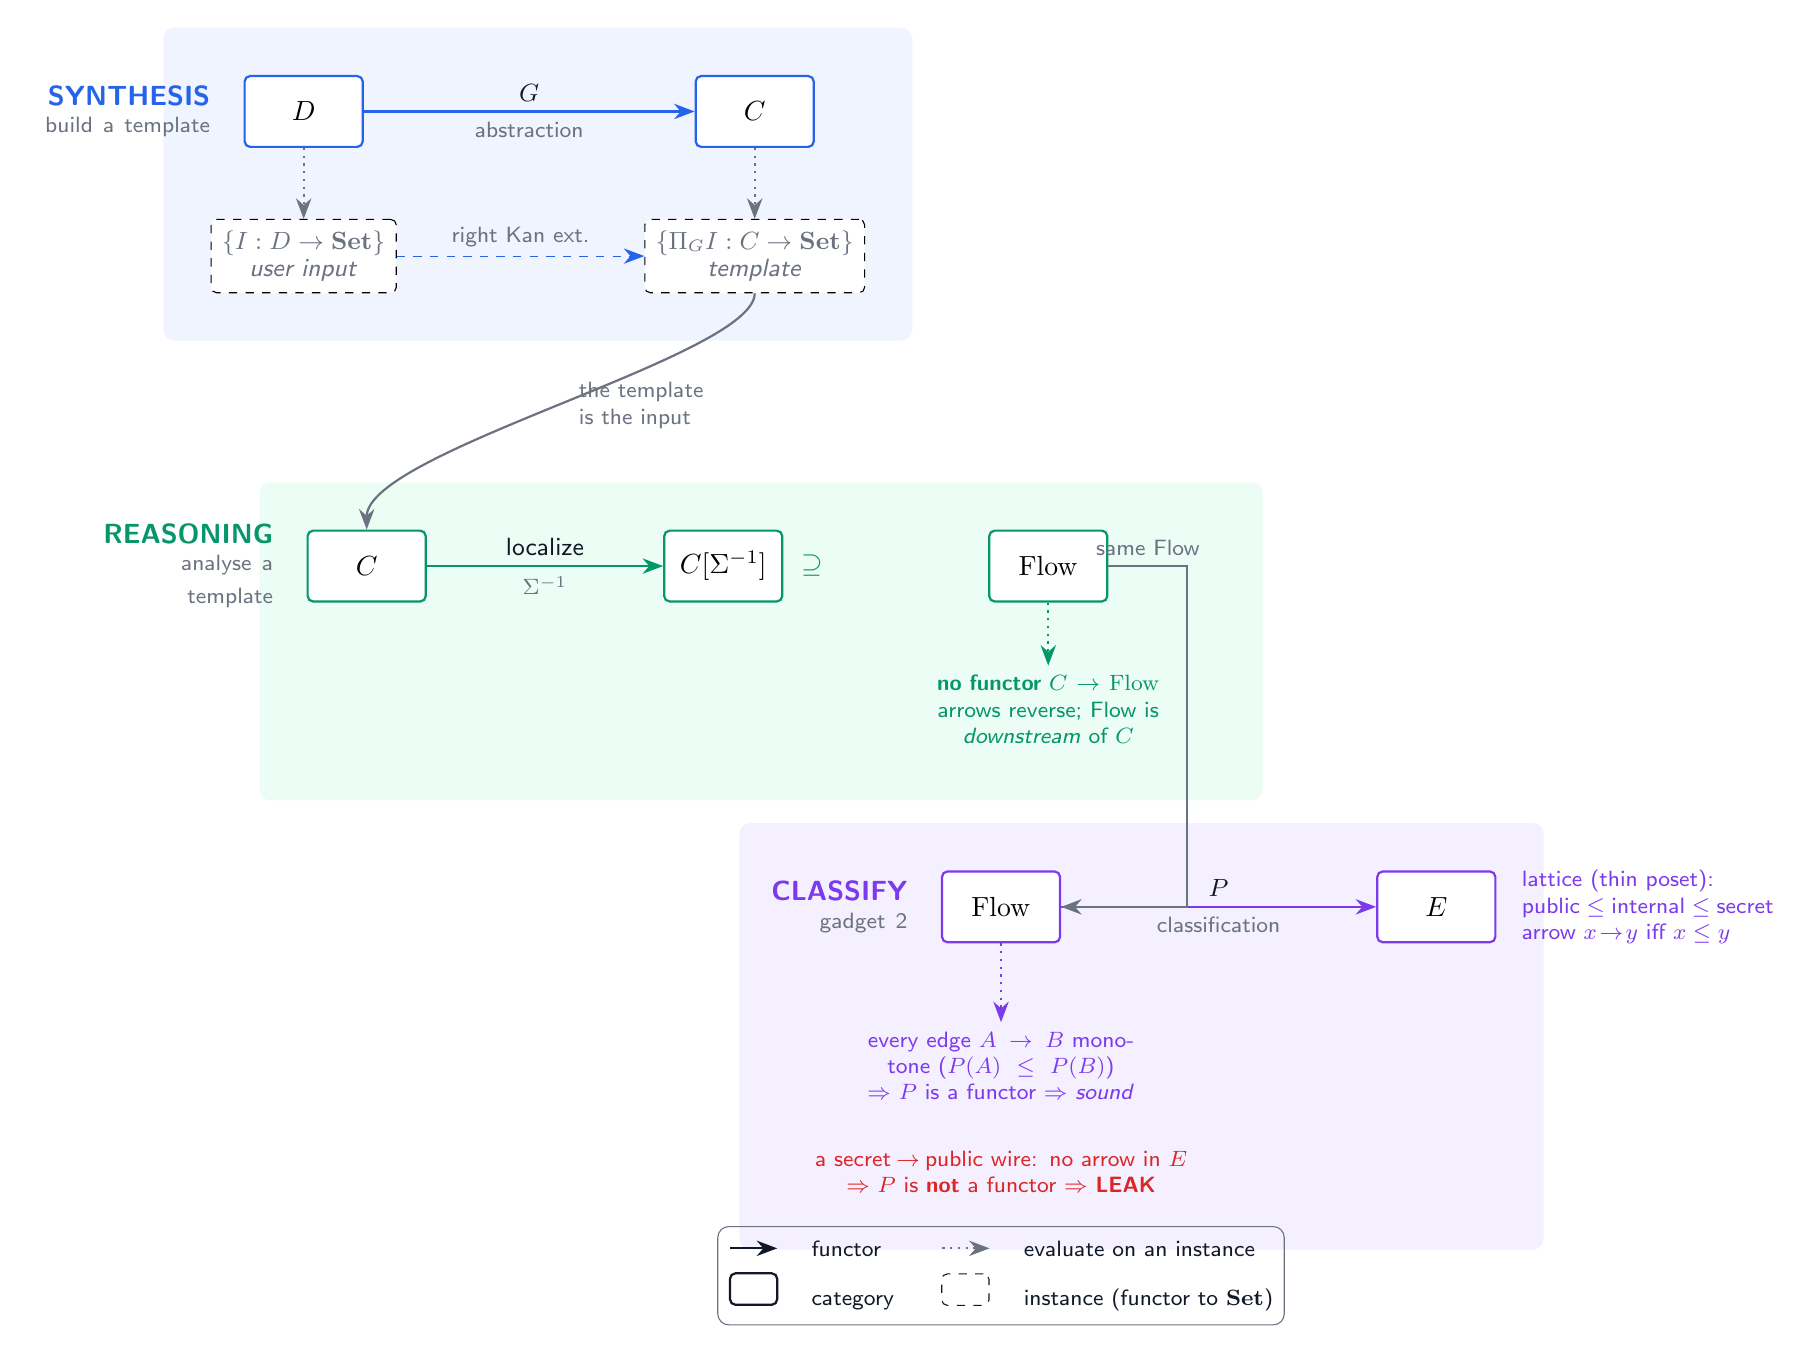
\begin{tikzpicture}[
  >={Stealth[length=2.6mm]},
  font=\sffamily,
  cat/.style={draw, rounded corners=2pt, minimum height=9mm, minimum width=15mm,
              inner sep=5pt, thick, fill=white, font=\sffamily},
  inst/.style={draw, dashed, rounded corners=2pt, fill=white, inner sep=4pt,
               align=center, font=\sffamily\small, text=mute},
  func/.style={->, thick},
  eval/.style={->, dotted, thick, mute},
  lbl/.style={font=\sffamily\small, text=ink},
  slbl/.style={font=\sffamily\footnotesize, text=mute},
  band/.style={font=\sffamily\bfseries},
]

% ============================================================ SYNTHESIS
\node[cat, draw=synth] (D) {$D$};
\node[cat, draw=synth, right=42mm of D] (Csyn) {$C$};
\draw[func, synth] (D) -- node[lbl, above]{$G$} node[slbl, below]{abstraction} (Csyn);

\node[inst, below=9mm of D]    (I)   {$\{I : D\to\Set\}$\\[-1pt]\emph{user input}};
\node[inst, below=9mm of Csyn] (PGI) {$\{\Pi_G I : C\to\Set\}$\\[-1pt]\emph{template}};
\draw[eval] (D) -- (I);
\draw[eval] (Csyn) -- (PGI);
\draw[->, dashed, synth] (I) -- node[slbl, above]{right Kan ext.} (PGI);

\node[band, synth, left=3mm of D, align=right, text width=22mm] {SYNTHESIS\\[-2pt]\textcolor{mute}{\footnotesize\mdseries build a template}};

\begin{scope}[on background layer]
  \node[fit=(D)(Csyn)(I)(PGI), rounded corners, fill=synthbg, inner sep=6mm] {};
\end{scope}

% ============================================================ REASONING
% place C again (the SAME C) as the hinge into reasoning
\node[cat, draw=reason, below=30mm of I, xshift=8mm] (Cre) {$C$};
\node[cat, draw=reason, right=30mm of Cre] (Loc) {$C[\Sigma^{-1}]$};
\node[cat, draw=reason, right=26mm of Loc] (Flow) {$\mathrm{Flow}$};

\draw[func, reason] (Cre) -- node[lbl, above]{localize} node[slbl, below]{$\Sigma^{-1}$} (Loc);
\node[reason, right=1mm of Loc] {$\supseteq$};

\node[band, reason, left=3mm of Cre, align=right, text width=22mm] {REASONING\\[-2pt]\textcolor{mute}{\footnotesize\mdseries analyse a template}};

% hinge: output of synthesis IS input of reasoning
\draw[->, thick, mute] (PGI.south) .. controls +(0,-8mm) and +(0,10mm) .. (Cre.north)
  node[slbl, midway, right, align=left, xshift=1mm]{the template\\is the input};

% note under Flow: no functor C->Flow
\node[slbl, below=8mm of Flow, align=center, text width=40mm, text=reason] (nof)
  {\textbf{no functor $C\!\to\!\mathrm{Flow}$}\\ arrows reverse; Flow is\\ \emph{downstream} of $C$};
\draw[eval, reason] (Flow) -- (nof);

\begin{scope}[on background layer]
  \node[fit=(Cre)(Flow)(nof), rounded corners, fill=reasonbg, inner sep=6mm] (rebox) {};
\end{scope}

% ============================================================ CLASSIFICATION
\node[cat, draw=classc, below=34mm of Flow, xshift=-6mm] (Flow2) {$\mathrm{Flow}$};
\node[cat, draw=classc, right=40mm of Flow2] (E) {$E$};
\draw[func, classc] (Flow2) -- node[lbl, above]{$P$} node[slbl, below]{classification} (E);

\node[band, classc, left=3mm of Flow2, align=right, text width=22mm] {CLASSIFY\\[-2pt]\textcolor{mute}{\footnotesize\mdseries gadget 2}};

% E internals: the lattice as a thin poset
\node[slbl, right=2mm of E, align=left, text=classc]
  {lattice (thin poset):\\ $\mathsf{public}\le\mathsf{internal}\le\mathsf{secret}$\\ arrow $x\!\to\!y$ iff $x\le y$};

% the good vs bad edge under P
\node[slbl, below=10mm of Flow2, align=center, text width=52mm, text=classc] (good)
  {every edge $A\!\to\!B$ monotone ($P(A)\!\le\!P(B)$)\\ $\Rightarrow$ $P$ is a functor $\Rightarrow$ \emph{sound}};
\node[slbl, below=4mm of good, align=center, text width=52mm, text=leak] (bad)
  {a $\mathsf{secret}\!\to\!\mathsf{public}$ wire: no arrow in $E$\\ $\Rightarrow$ $P$ is \textbf{not} a functor $\Rightarrow$ \textbf{LEAK}};
\draw[eval, classc] (Flow2) -- (good);

\begin{scope}[on background layer]
  \node[fit=(Flow2)(E)(good)(bad), rounded corners, fill=classbg, inner sep=6mm] {};
\end{scope}

% connect Flow (reasoning) down to Flow (classify) — routed down the right,
% clear of the "no functor" note, and drawn last so it sits above band fills.
\draw[->, thick, mute] (Flow.east) -- ++(10mm,0)
  node[slbl, midway, above]{same Flow}
  |- (Flow2.east);

% ============================================================ LEGEND
\node[slbl, below=3mm of bad, align=left, text=ink, draw=mute, rounded corners, inner sep=4pt] {
  \begin{tabular}{@{}l l @{\hskip 6mm} l l@{}}
  \tikz{\draw[func,ink] (0,0)--(6mm,0);} & functor &
  \tikz{\draw[eval,mute] (0,0)--(6mm,0);} & evaluate on an instance \\[3pt]
  \tikz{\node[cat,minimum width=6mm,minimum height=4mm]{};} & category &
  \tikz{\node[inst,minimum width=6mm,minimum height=4mm]{};} & instance (functor to $\Set$) \\
  \end{tabular}};

\end{tikzpicture}
\end{document}
